\documentclass[a4paper,12pt]{article}
\usepackage [utf8x]{inputenc}
\usepackage[czech]{babel}
\usepackage{graphicx}
\usepackage{amsmath}
\usepackage{siunitx}
\usepackage{xspace}
\usepackage{url}
\usepackage{indentfirst}
\usepackage[margin=22mm]{geometry}
\usepackage{esvect}
\usepackage{ragged2e}
\usepackage{tikz,pgf}
\usepackage{bm}
\usepackage{perpage}
\usepackage{capt-of}

\graphicspath{
	{img/}
	{plots/}
}

\MakeSorted{figure}
\newtoks\jmenopraktika \newtoks\jmeno \newtoks\datum
\newtoks\obor \newtoks\skupina \newtoks\rocnik \newtoks\semestr
\newtoks\cisloulohy \newtoks\jmenoulohy
\newtoks\tlak \newtoks\teplota \newtoks\vlhkost
\jmenopraktika={Praktikum v~čistých prostorách}  % nahradte jmenem vaseho predmetu
\jmeno={Radek Horňák, Lukáš Vrána}            
\datum={29. 4. 2022}        % nahradte datem mereni ulohy
\obor={F}                     
\skupina={Pá 7:30}            
\rocnik={2.}                  
\semestr={IV.}                 
\cisloulohy={6}    % cislo ulohy           

\begin{document}
	\begin{center}
		{\Large Přírodovědecká fakulta Masarykovy univerzity} \\
		\bigskip
		{\Large \bfseries EXPERIMENTÁLNÍ METODY 2} \\
		\bigskip
		{\Large \the\jmenopraktika}
	\end{center}
	\bigskip
	\noindent
	\setlength{\arrayrulewidth}{1pt}
	\begin{tabular*}{\textwidth}{@{\extracolsep{\fill}} l l}
		\large {\bfseries Zpracovali:}  \the\jmeno  \hspace{9mm} \large  
		{\bfseries Naměřeno:} \the\datum\\[2.5mm]
		\large  {\bfseries Obor:}  \the\obor \hspace{81mm} {\bfseries Skupina:} \the\skupina \\
		\hline
	\end{tabular*}

\section{Úvod}
Fotolitografie je hojně využívaná metoda pro výrobu desek plošných spojů. 
Slouží k~pře\-no\-su motivu z~fotomasky na substrát a tvoří tak společně 
s~leptáním 
a depozicemi tenkých vrstev výrobní proces nejrůznějších polovodičových 
struktur. Mezi ně patří i integrované obvody, které dále tvoří například čipy a 
paměti. Veškerý fotolitografický proces se musí odehrávat v~kontrolovaném 
prostředí, které nazýváme čisté prostory. Jsou zde požadavky na maximální počet 
částic pevného aerosolu o~určité velikosti. Hlavním důvodem je, že 
nekontrolované prostředí by vedlo k~defektům v~připravovaných strukturách pohybujících se v~rozměrech \si{\micro\meter} až \si{\nano\meter}.

\section{Praktická část}
Naším vstupním substrátem byla křemíková deska, na níž byla oxidací vytvořená 
dielektrická vrstva SiO$_2$ a následně na ni naprášena vrstva hliníku. Prvním 
krokem našeho fotolitografického procesu bylo nanesení pozitivního 
fotocitlového laku metodou spin coating. Substrát se umístil na disk, který může 
rotovat. Na substrát se kápnul tekutý lak, který se při rotaci odstředivými 
silami rovnoměrně rozlil po povrchu. Rotace o~rychlosti 3000\,ot./min trvala 
30 sekund. Vzniklá vrstva je vidět na obr.~\ref{1spincoating}.

Dalším krokem bylo zahřátí desky s~nanesenou vrstvou, tzv. soft bake, po dobu 3 
minut na 85 -- 90\,$^{\circ}$C, viz obr.~\ref{2bake}. Takto vytvrzenou vrstvu 
jsme nechali další 3 minuty vychladnout.

Následoval osvit UV světlem ve fotolitografu. Maska v~poměru 1:1 obsahovala 
mimo jiné různé rezistory a kondenzátory. Samotný přístroj je vidět na 
obr.~\ref{3osvit}. Jednalo se o~automatizovaný proces. Jelikož jsme v~prvním 
kroku 
nanesli na substrát pozitivní fotocitlivý lak, na osvícených místech došlo
k~porušení struktury fotolaku.

Dále jsme provedli vyvolání přeneseného motivu masky. To spočívalo v~chemickém 
odleptání osvíceného fotolaku ve vývojce po několik minut a následném oplachu 
demineralizovanou vodou, viz obr.~\ref{4vyvolani}. 

Na obr.~\ref{5odstredeni} je vidět odstředivka, pomocí které jsme v~dalším 
kroku mokrou desku osušili. Poté jsme mohli pod mikroskopem zkontroloval 
kvalitu vyvolaného motivu.

Po usušení na odstředivce jsme provedli tzv. hard bake, tedy zahřátí desky na 
110 -- 115\,$^{\circ}$C po dobu 3 minut. Tento krok je vidět na 
obr.~\ref{7hardbake}.

\newpage
\begin{figure}[h!]
	\centering
	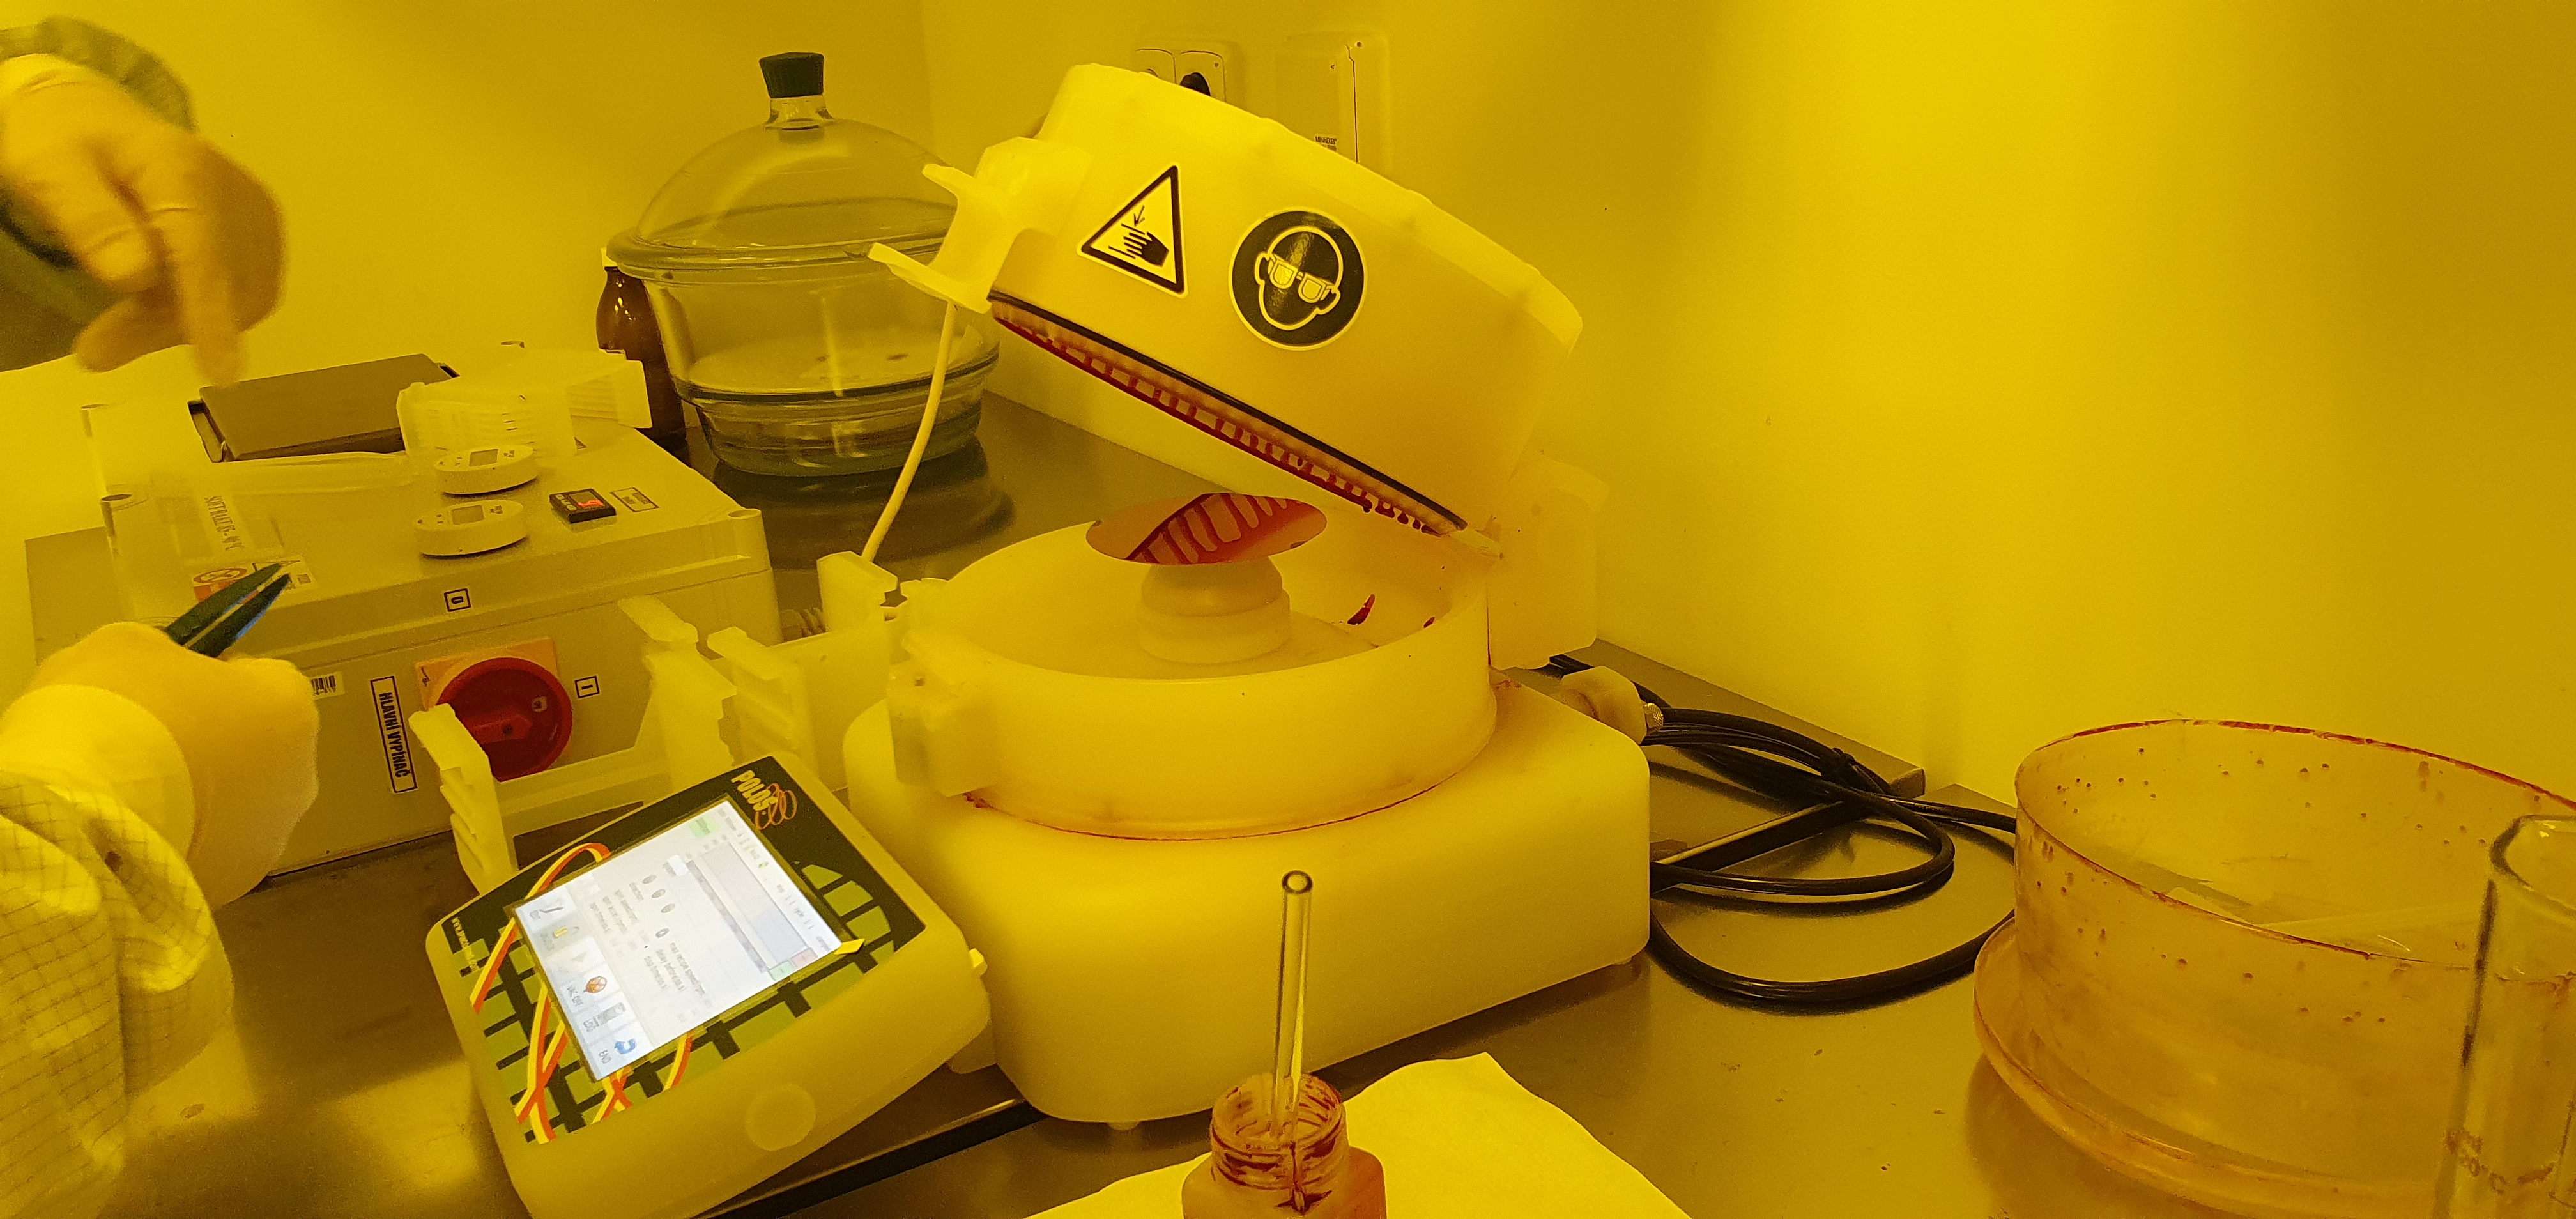
\includegraphics[width=130mm]{1spincoating.jpg}
	\caption{Nanesení fotolaku metodou spin coating}
	\label{1spincoating}
\end{figure}

\begin{figure}[h!]
	\centering
	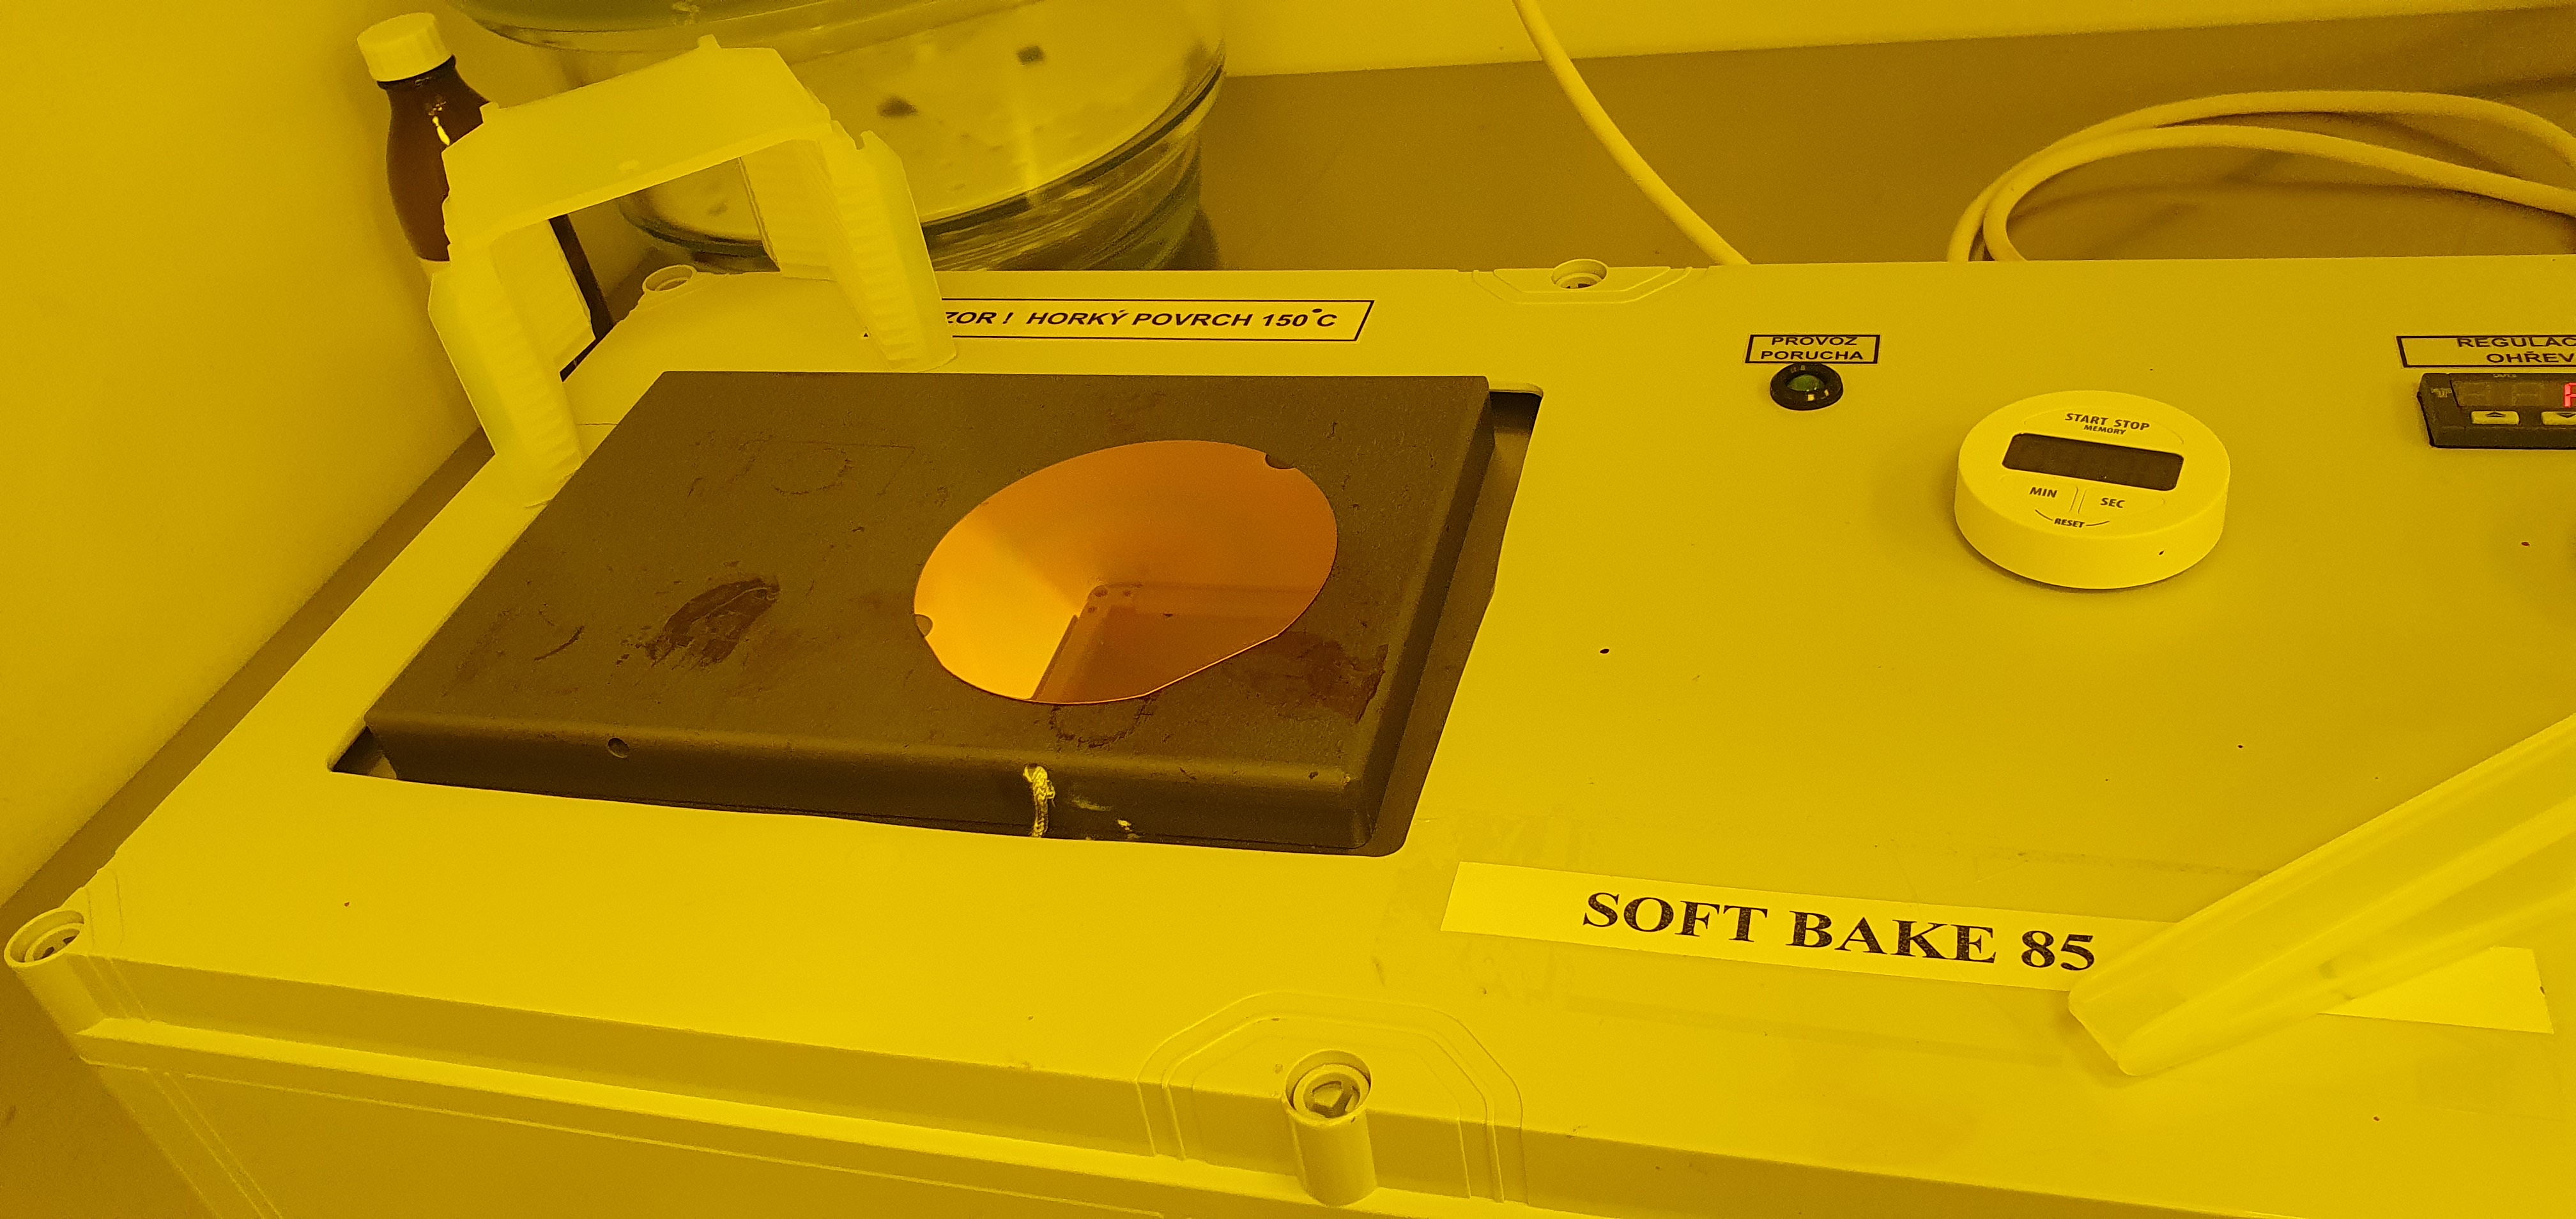
\includegraphics[width=130mm]{2bake.jpg}
	\caption{Soft bake}
	\label{2bake}
\end{figure}

\begin{figure}[h!]
	\centering
	\includegraphics[width=130mm]{3osvit.jpg}
	\caption{Osvit ve fotolitografu}
	\label{3osvit}
\end{figure}

\newpage
\begin{figure}[h!]
	\centering
	\includegraphics[width=130mm]{4vyvolani.jpg}
	\caption{Vyvolání osvícených míst}
	\label{4vyvolani}
\end{figure}

\begin{figure}[h!]
	\centering
	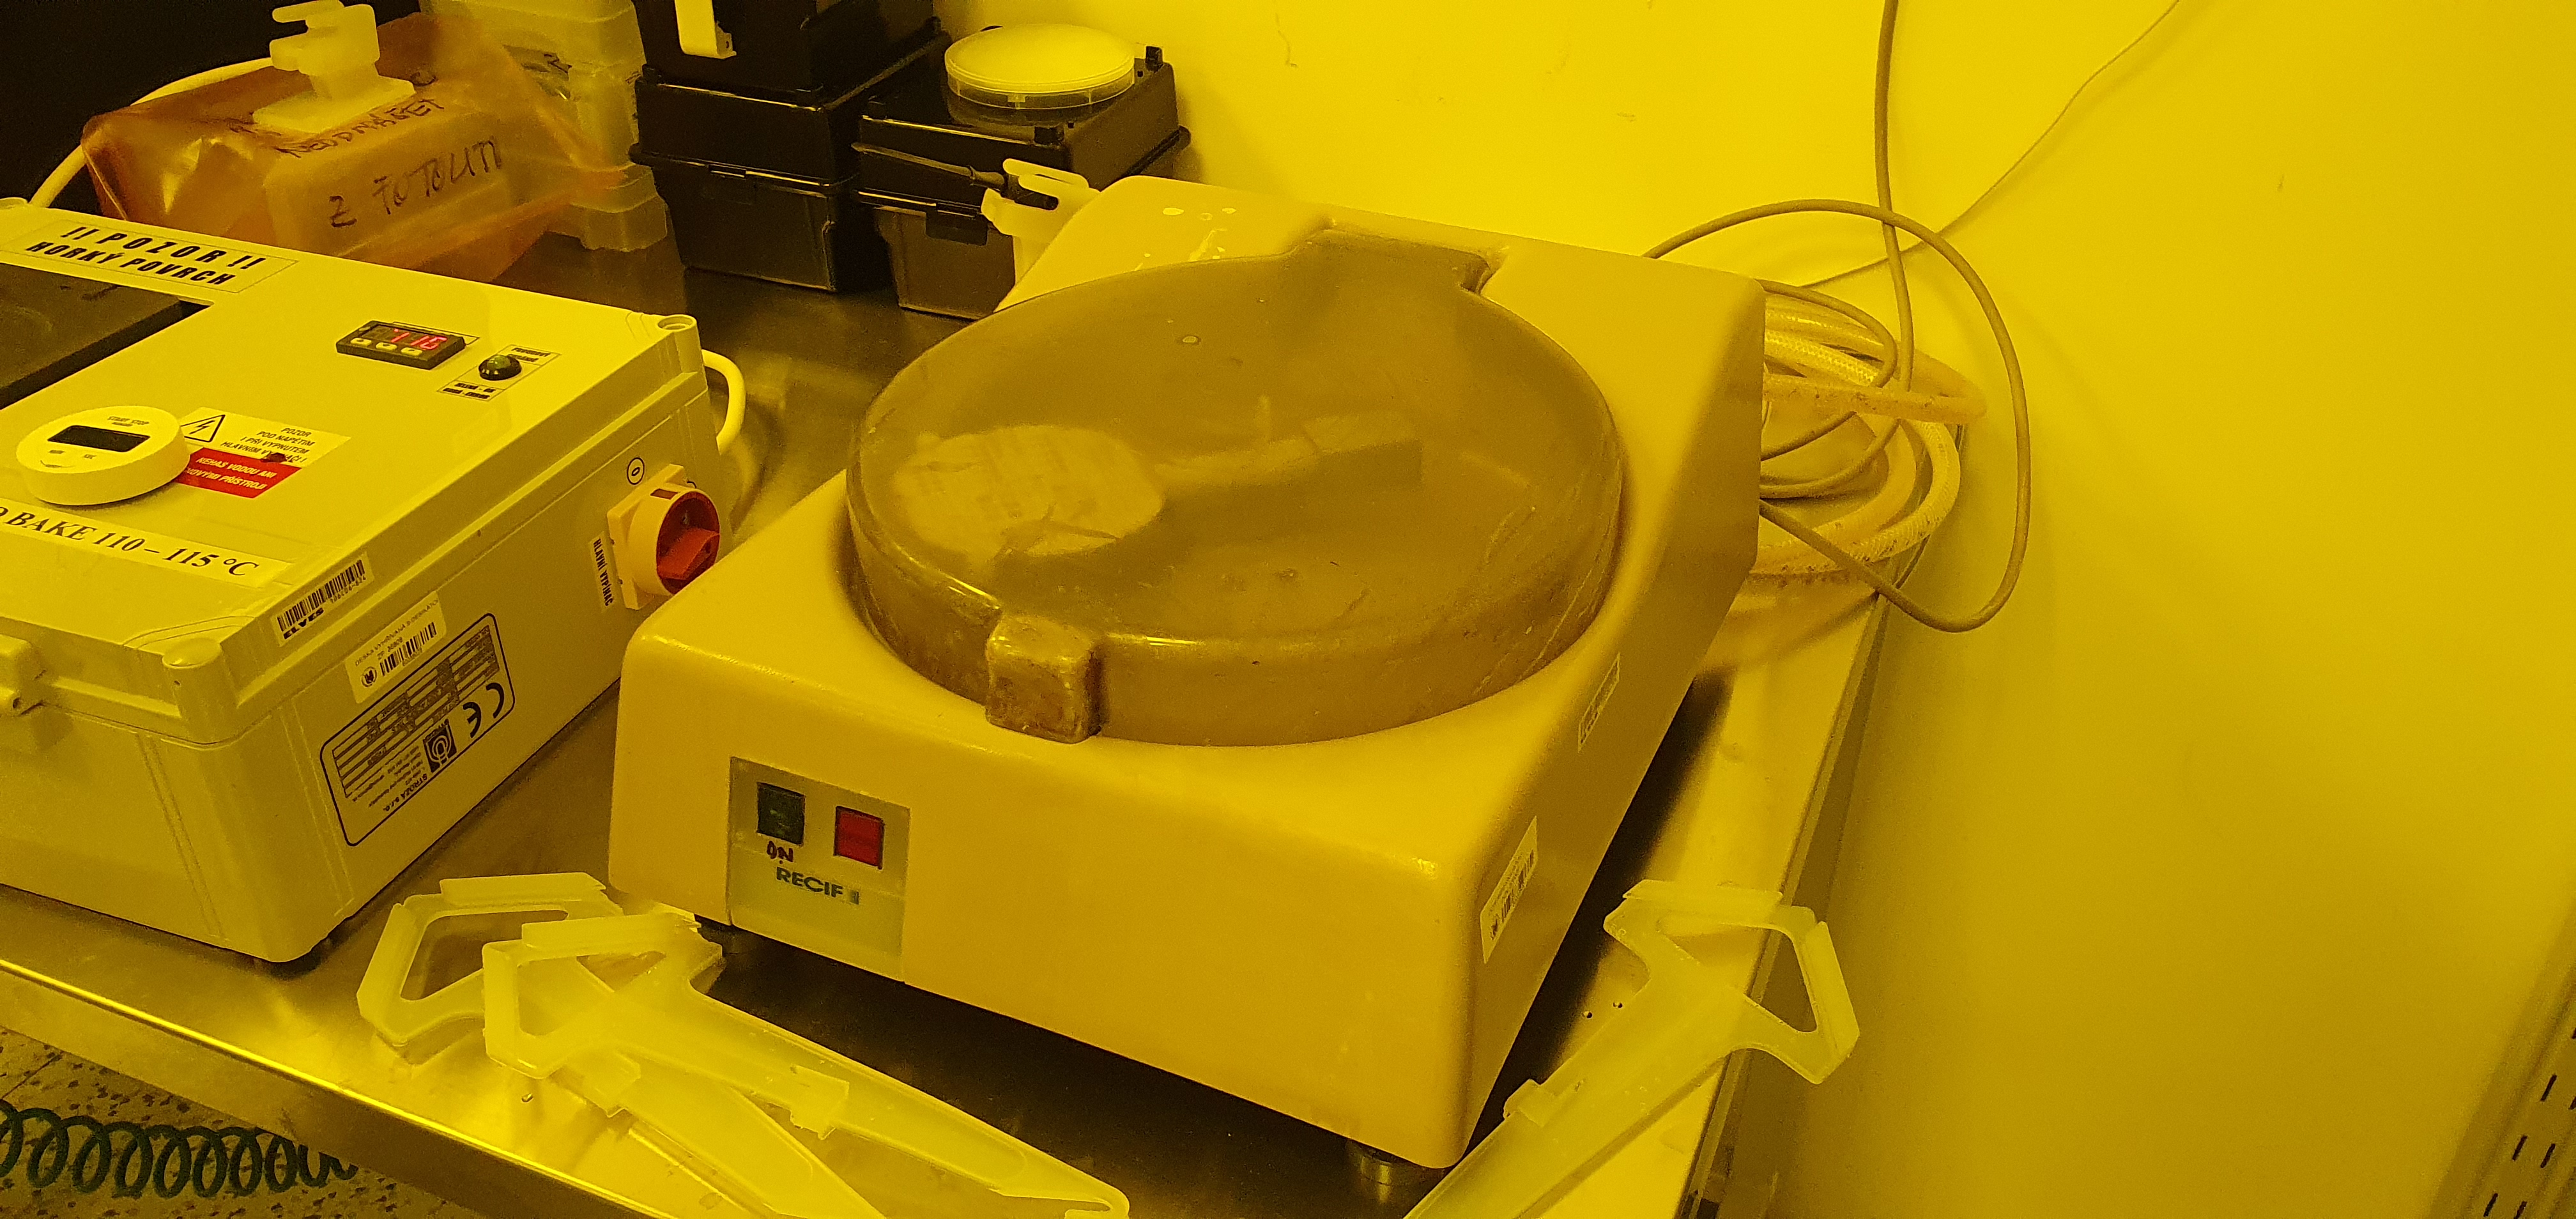
\includegraphics[width=130mm]{5odstredeni.jpg}
	\caption{Sušení na odstředivce}
	\label{5odstredeni}
\end{figure}

\begin{figure}[h!]
	\centering
	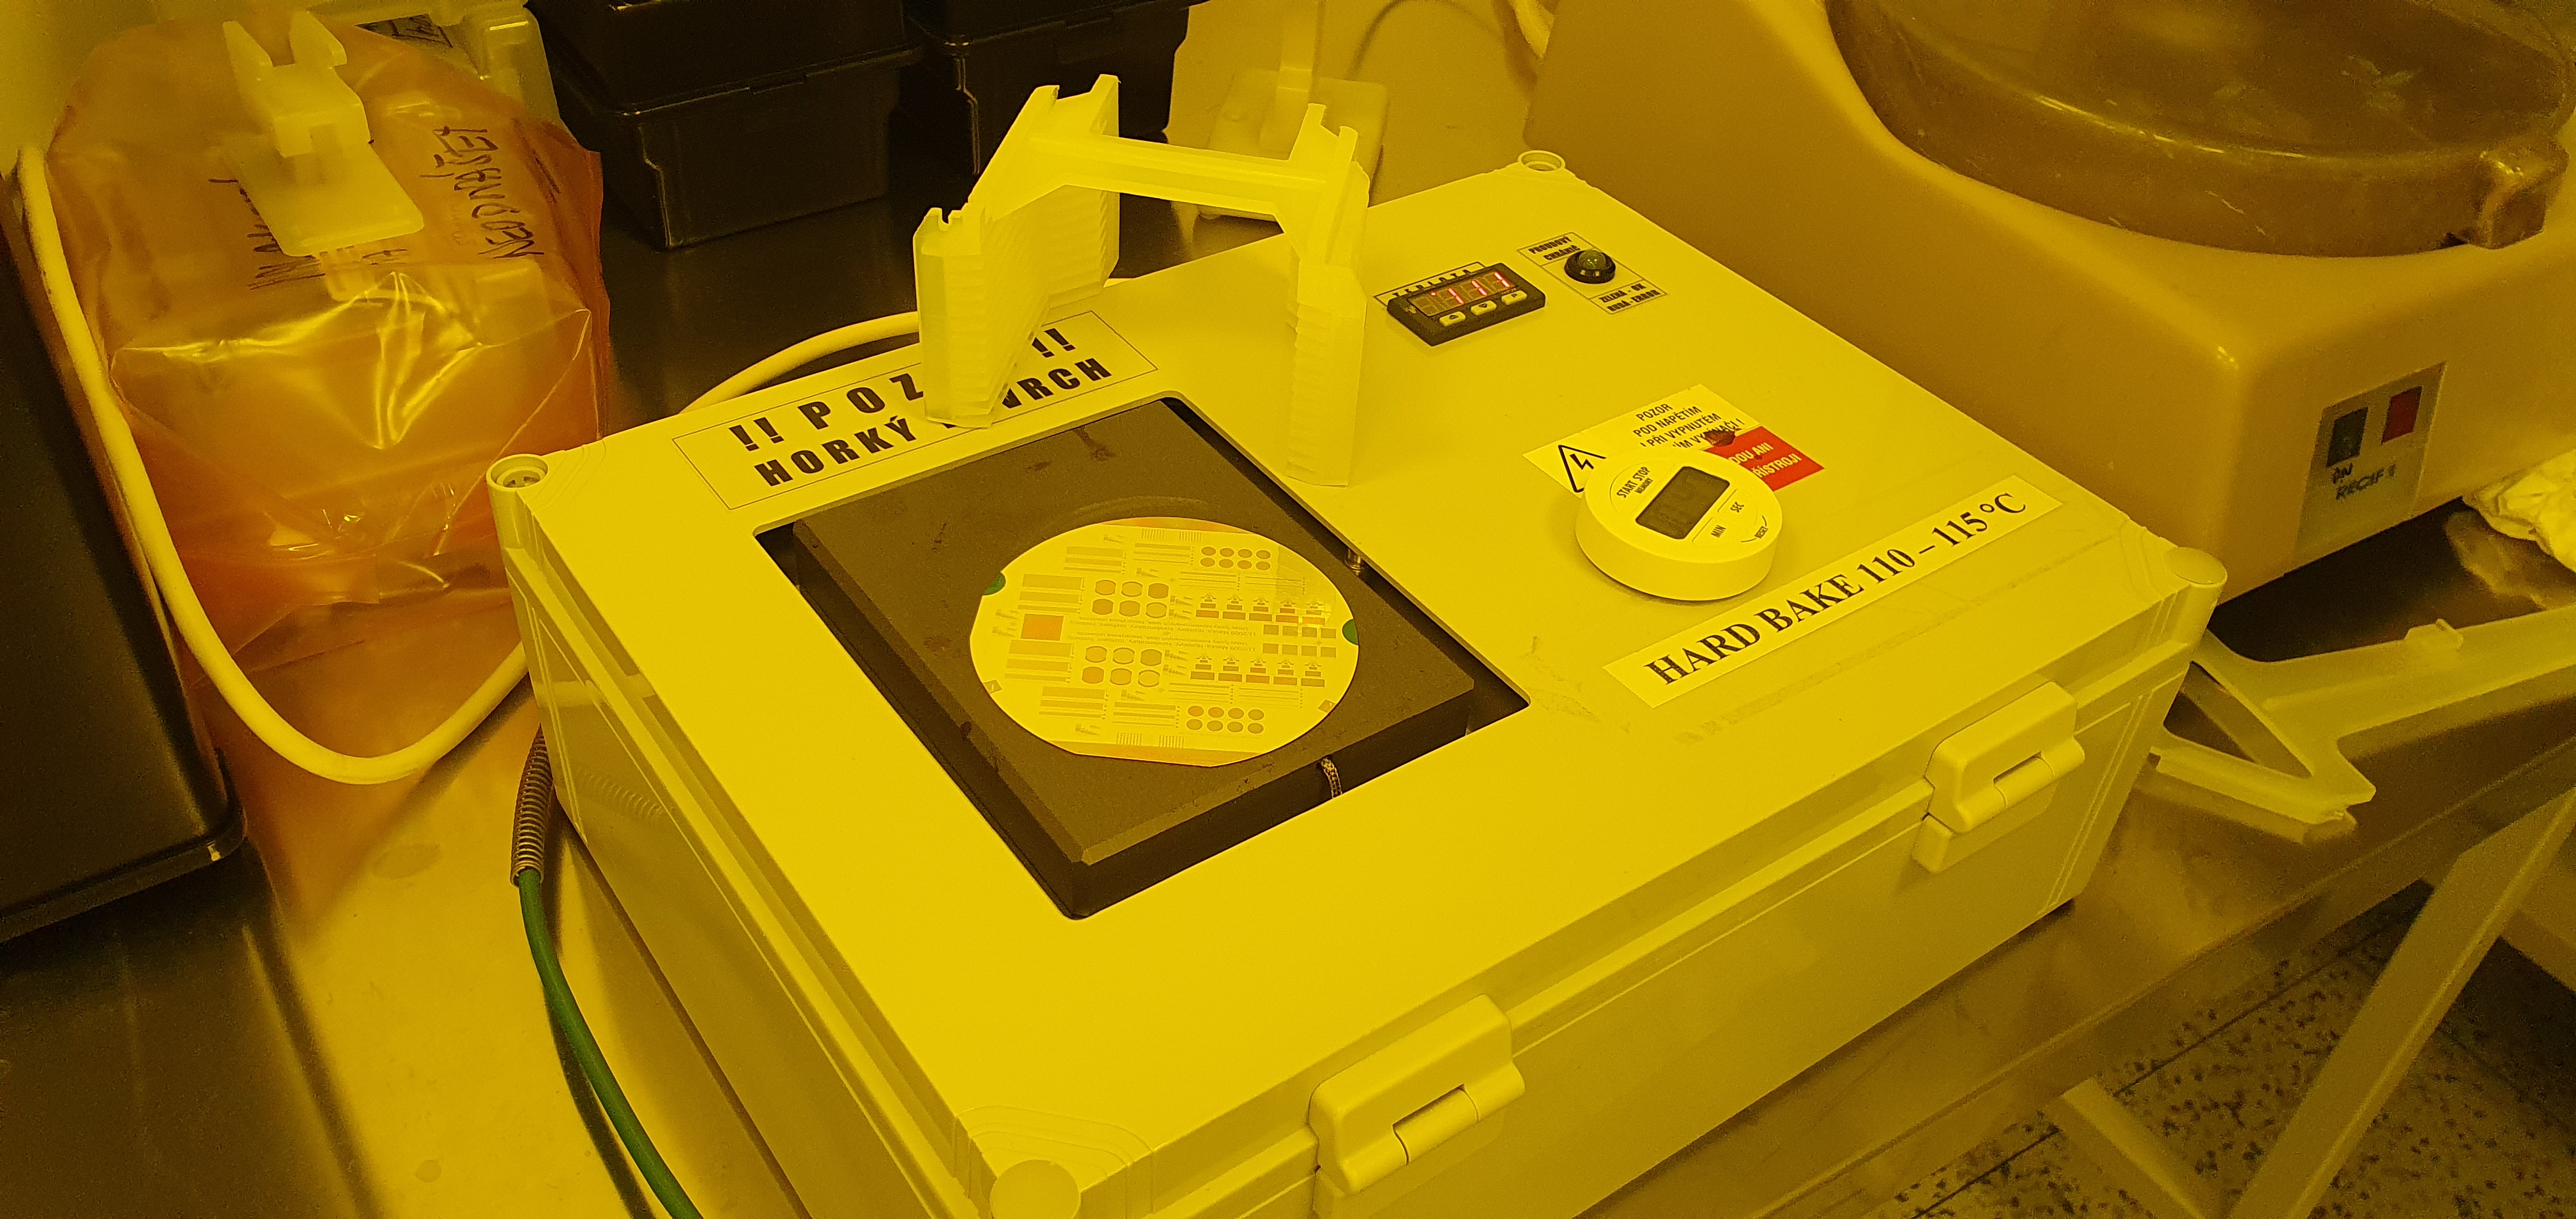
\includegraphics[width=130mm]{7hardbake.jpg}
	\caption{Hard bake}
	\label{7hardbake}
\end{figure}

\newpage
Jako další krok jsme provedli chemické odleptání hliníku na vyvolaných místech. 
To probíhalo 50 sekund a po něm následoval oplach desky ve vaničce i oplachovou 
sprchou, viz obr.~\ref{8Aletch}. Opět jsme desku usušili na odstředivce.

Posledním krokem v~našem procesu bylo smytí zbylého fotolaku v~acetonu a poté 
oplach v~isopropylalkoholu na stanovišti, které je vidět na 
obr.~\ref{11oplach}. Výslednou desku s~vytvořeným motivem můžeme vidět na 
obr.~\ref{deska}.

Na vytvořené desce jsme digitálním multimetrem naměřili odpory a kapacity 
některých rezistorů, respektive kondenzátorů. Schéma motivu je vidět na obr. 
\ref{mereni}. Rezistory označené 1,~2~a~3 mají odpory 382,6\,\si{\ohm}, 
450,6\,\si{\ohm} a 1,13\,\si{\kilo\ohm} v~tomto pořadí. Kondenzátory označené 1~a~2 mají kapacity 380\,\si{\pico\farad}, respektive 660\,\si{\pico\farad}.


\begin{figure}[h!]
	\centering
	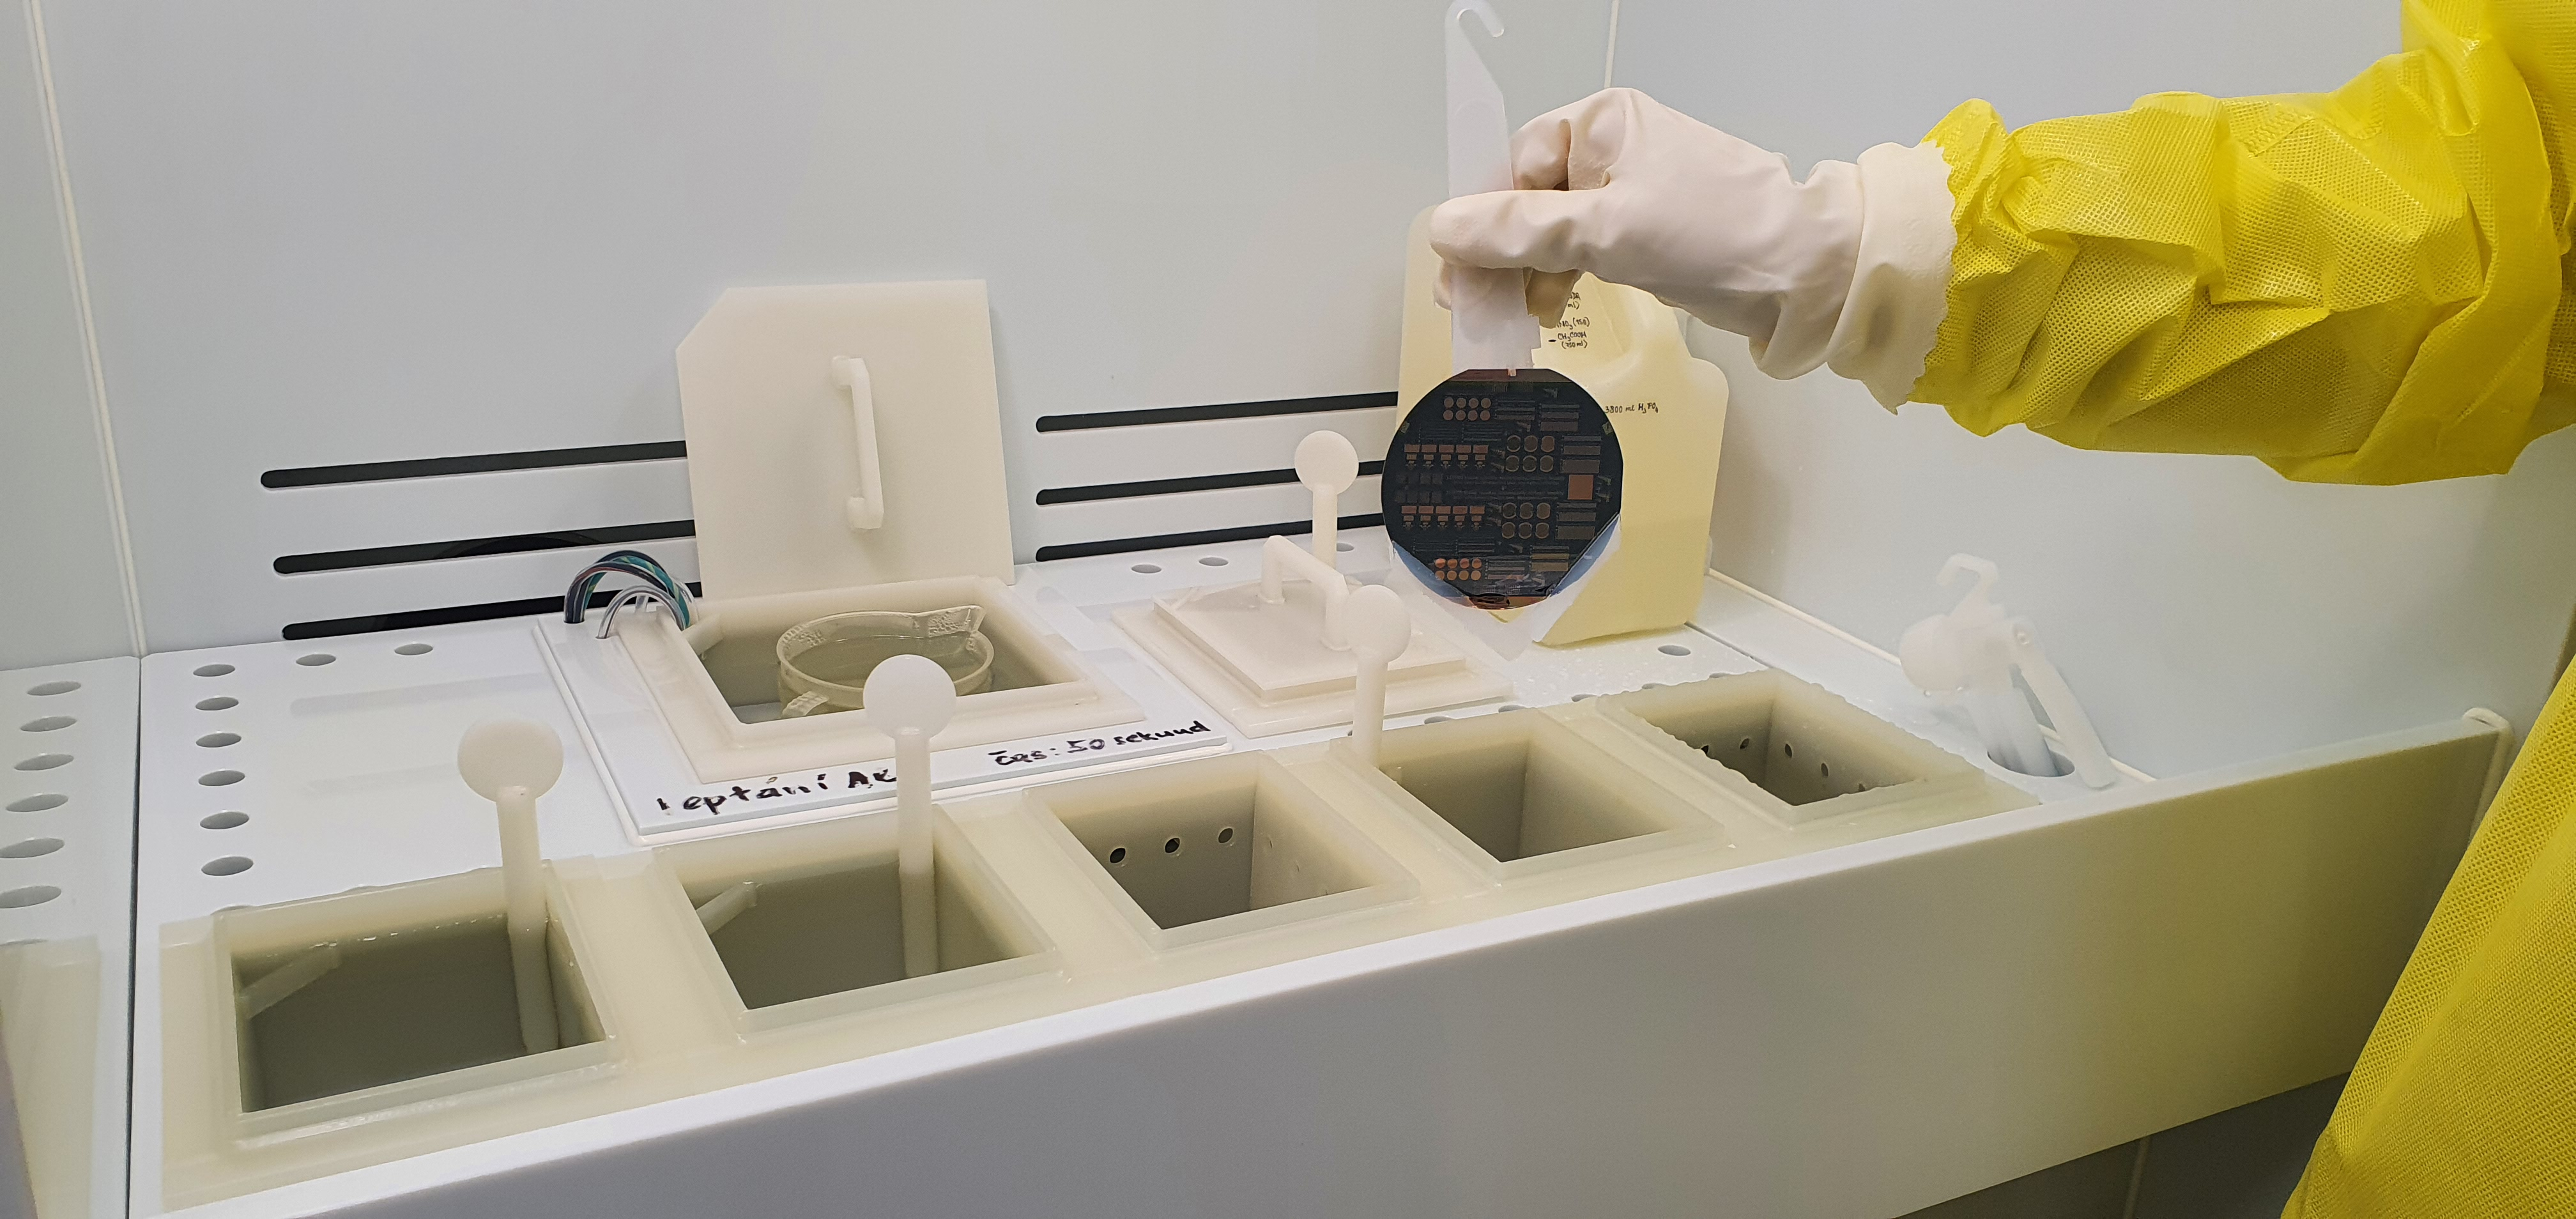
\includegraphics[width=130mm]{8Aletch.jpg}
	\caption{Leptání hliníku}
	\label{8Aletch}
\end{figure}

\begin{figure}[h!]
	\centering
	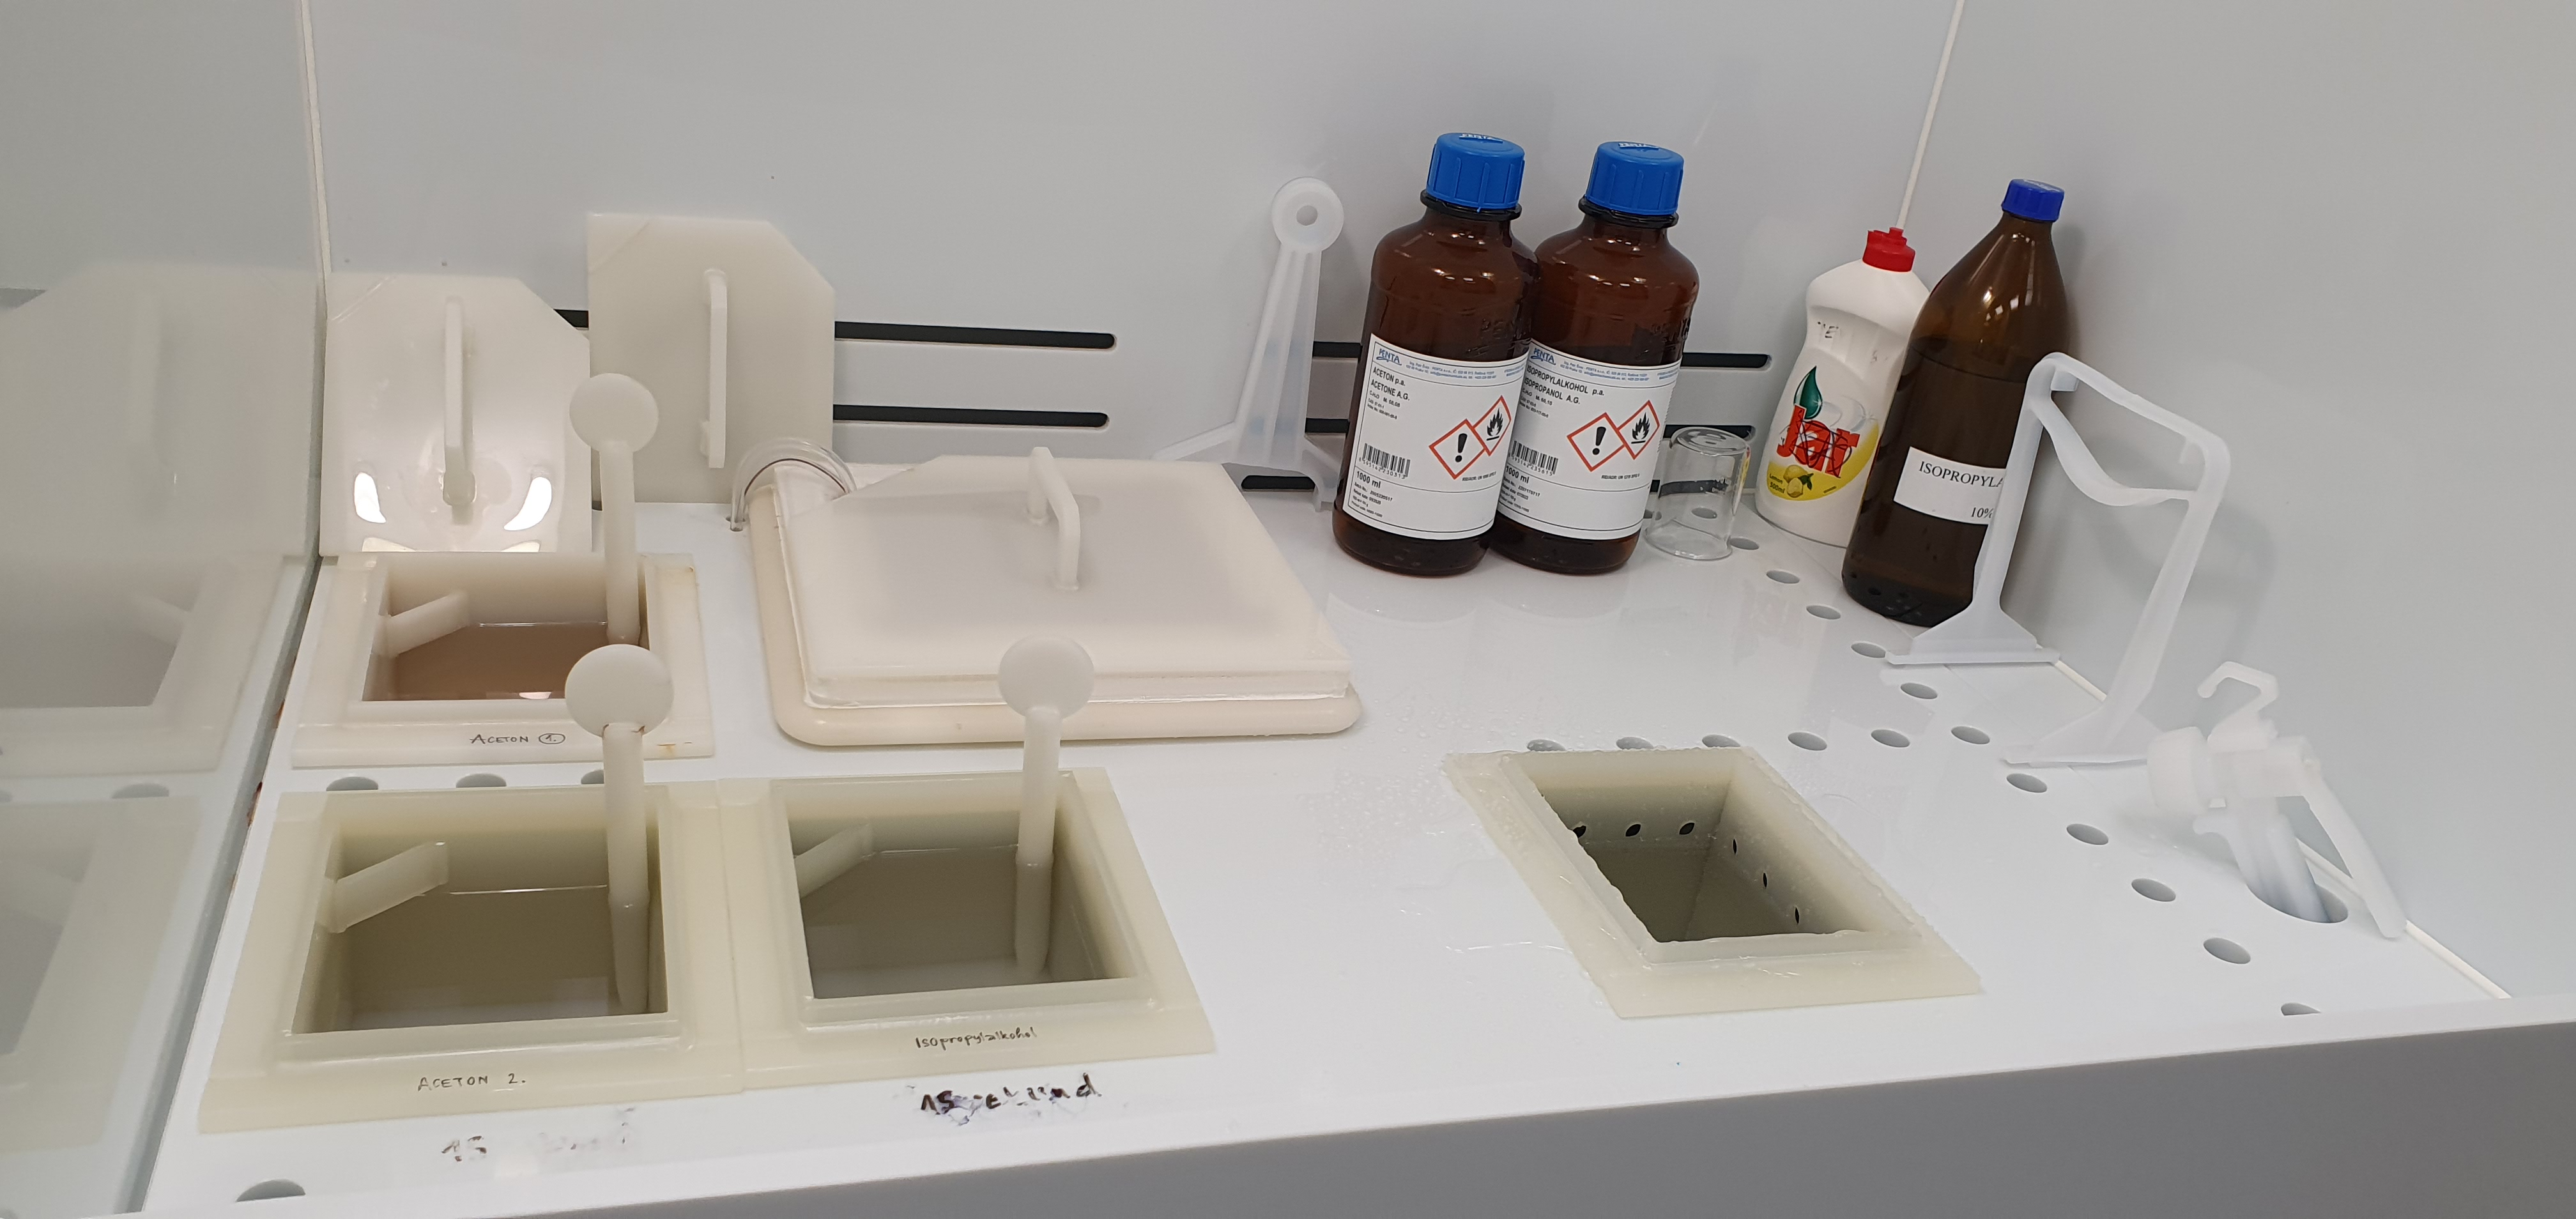
\includegraphics[width=130mm]{11oplach.jpg}
	\caption{Oplach fotolaku}
	\label{11oplach}
\end{figure}

\newpage
\begin{figure}[h!]
	\centering
	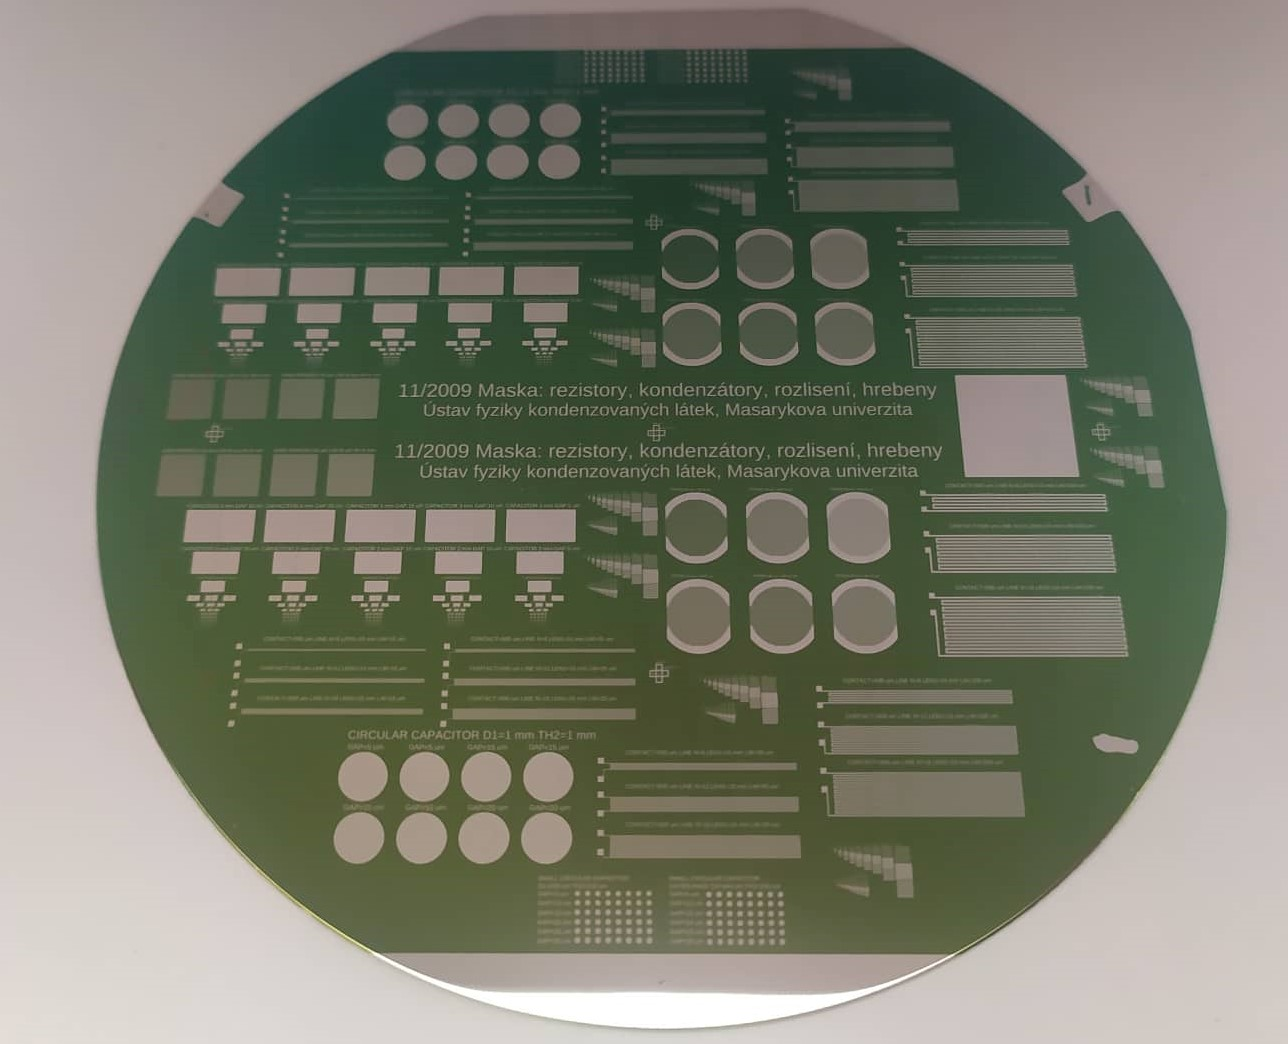
\includegraphics[width=130mm]{deska.jpg}
	\caption{Vyrobená deska s~motivem}
	\label{deska}
\end{figure}

\begin{figure}[h!]
	\centering
	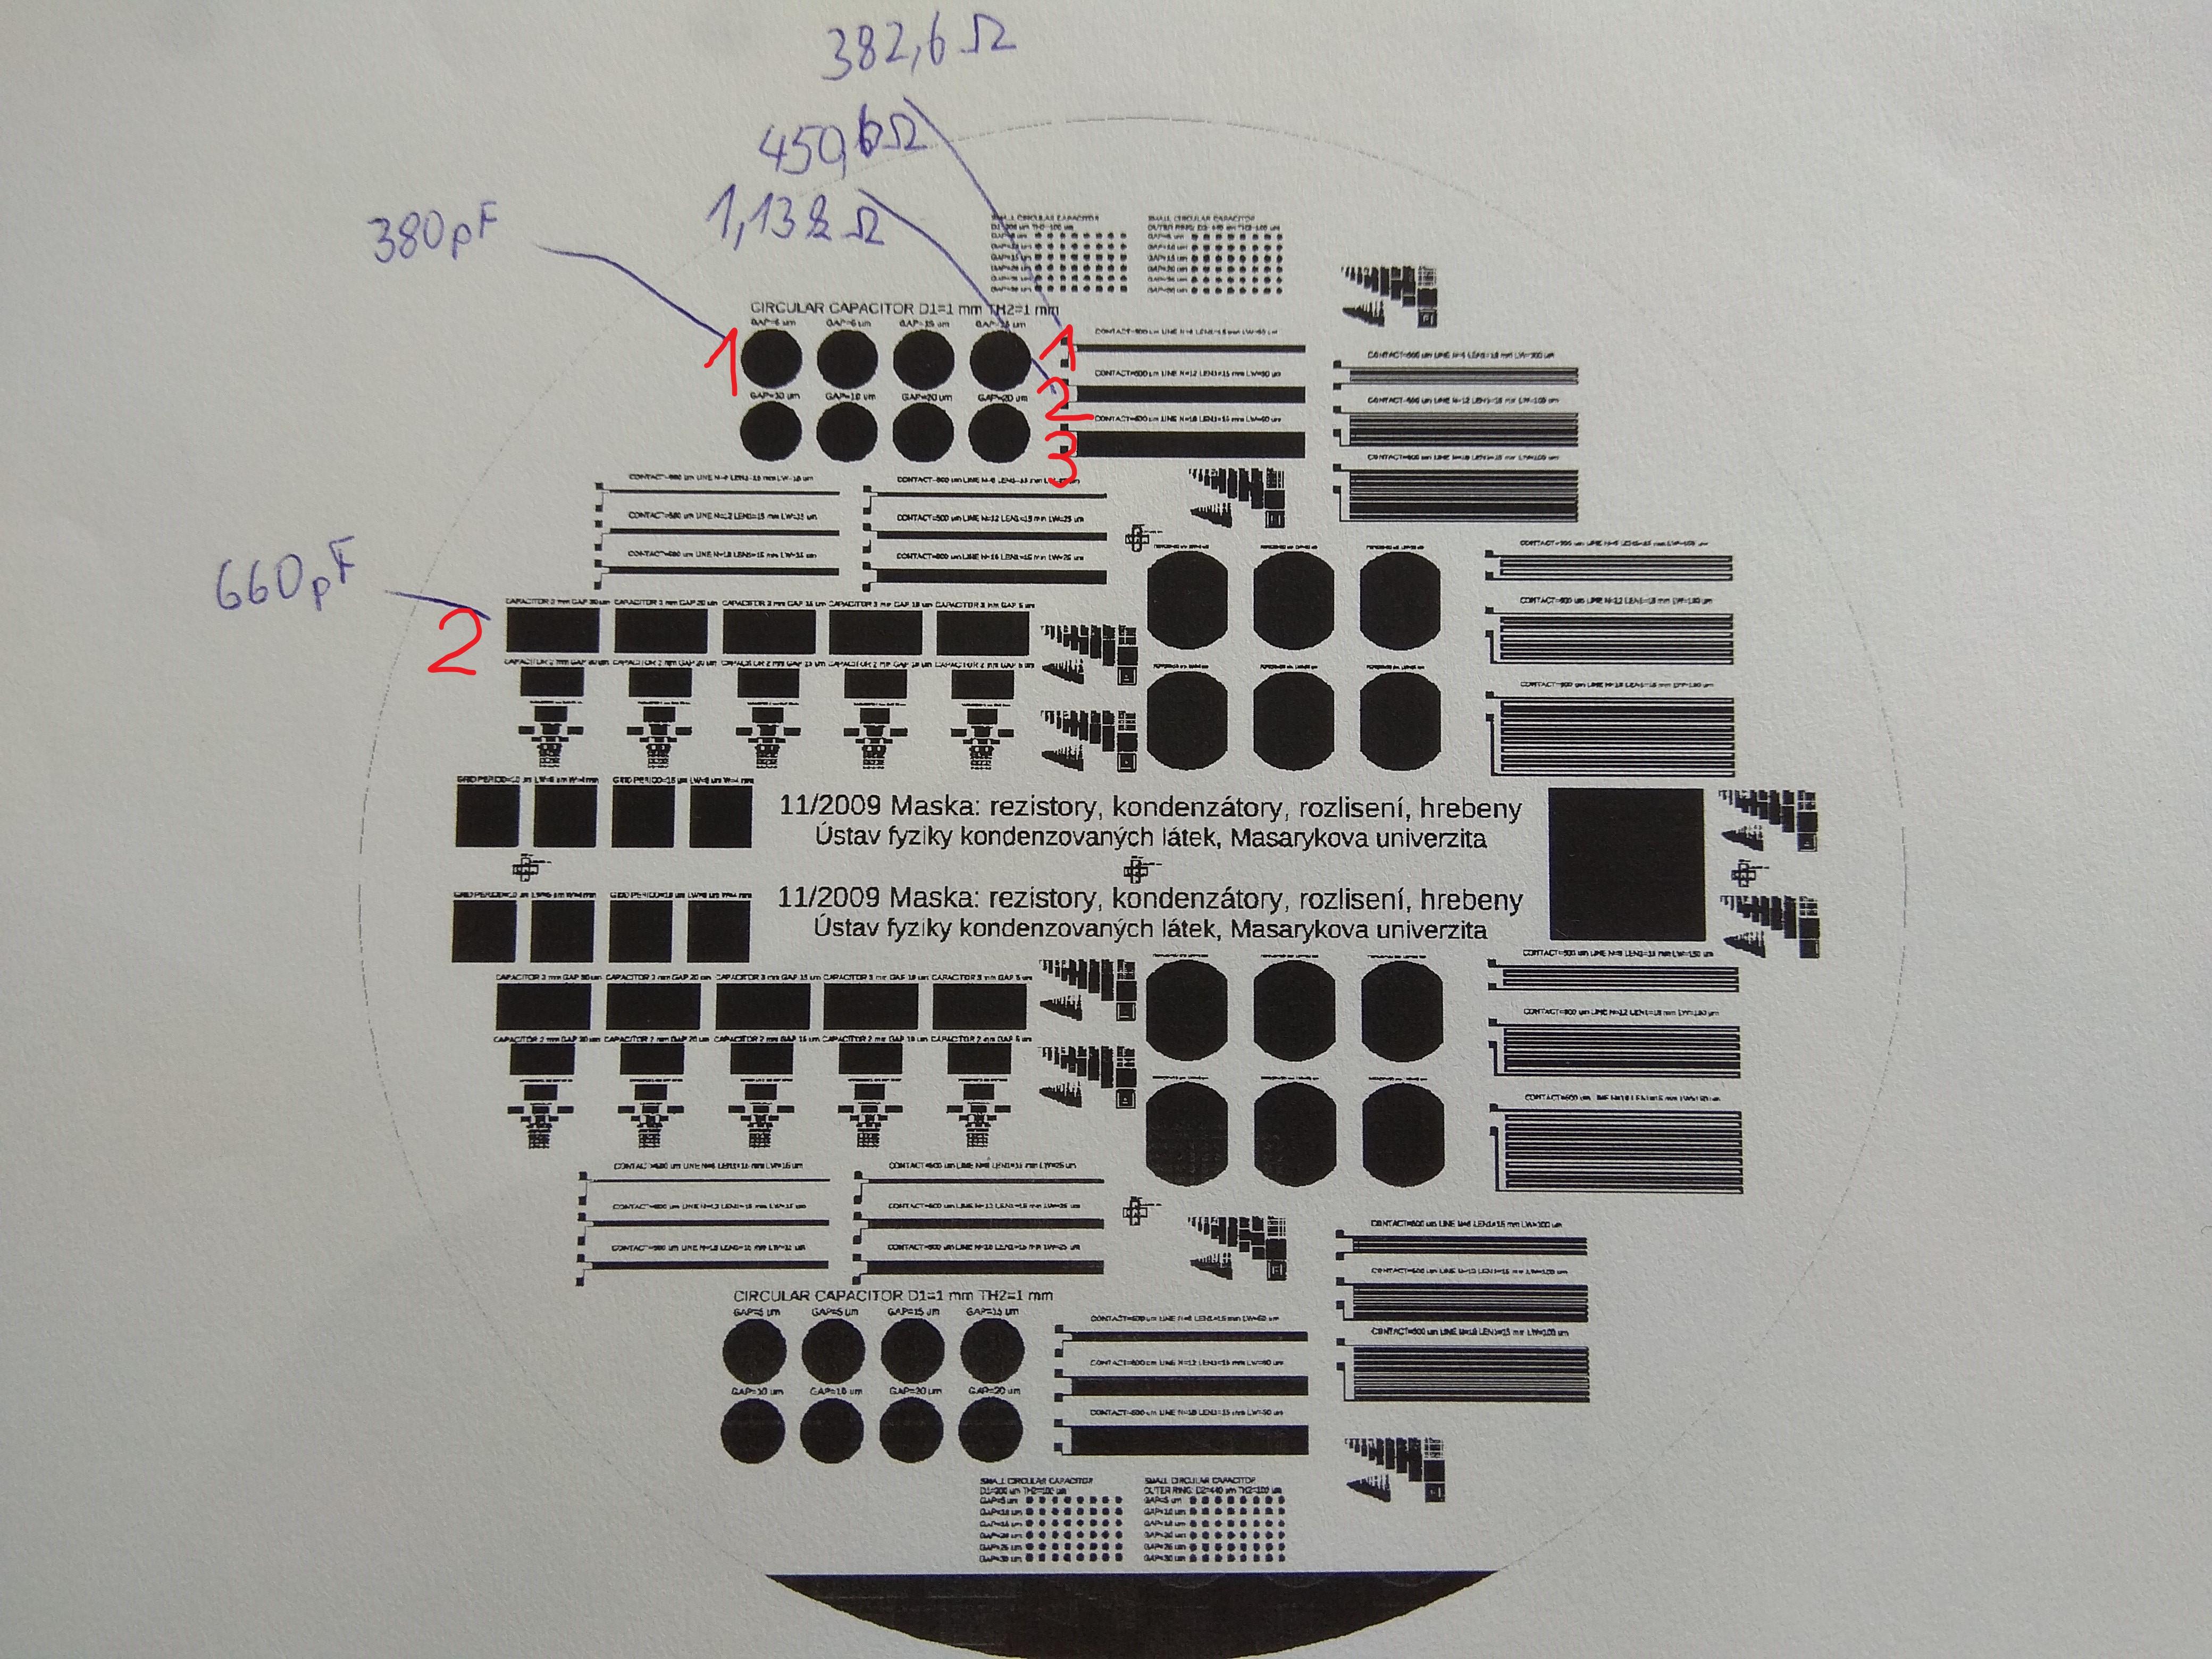
\includegraphics[width=130mm]{mereni.jpg}
	\caption{Schéma motivu}
	\label{mereni}
\end{figure}

\newpage
 Dále jsme interferometrem provedli měření tloušťky SiO$_2$ vrstvy, jehož 
 průběh je vidět na obr.~\ref{9interferometr}. Výsledná tloušťka se pohybovala 
 okolo 380\,\si{\nano\meter}. Nakonec jsme profilometrem zjišťovali výšku 
 hliníkového motivu, viz měření na obr.~\ref{10profilometr}. K~tomuto účelu 
 nemohl být použit interferometr, protože Al vrstva je neprůhledná. Profilometr 
 se svým hrotem je tedy v~tomto případě ideální na měření rozdílu výšky mezi 
 místem s~Al vrstvou a místem bez ní. Výsledná tloušťka hliníku na substrátu se 
 pohybuje kolem 250\,\si{\nano\meter}.
 
\begin{figure}[h!]
	\centering
	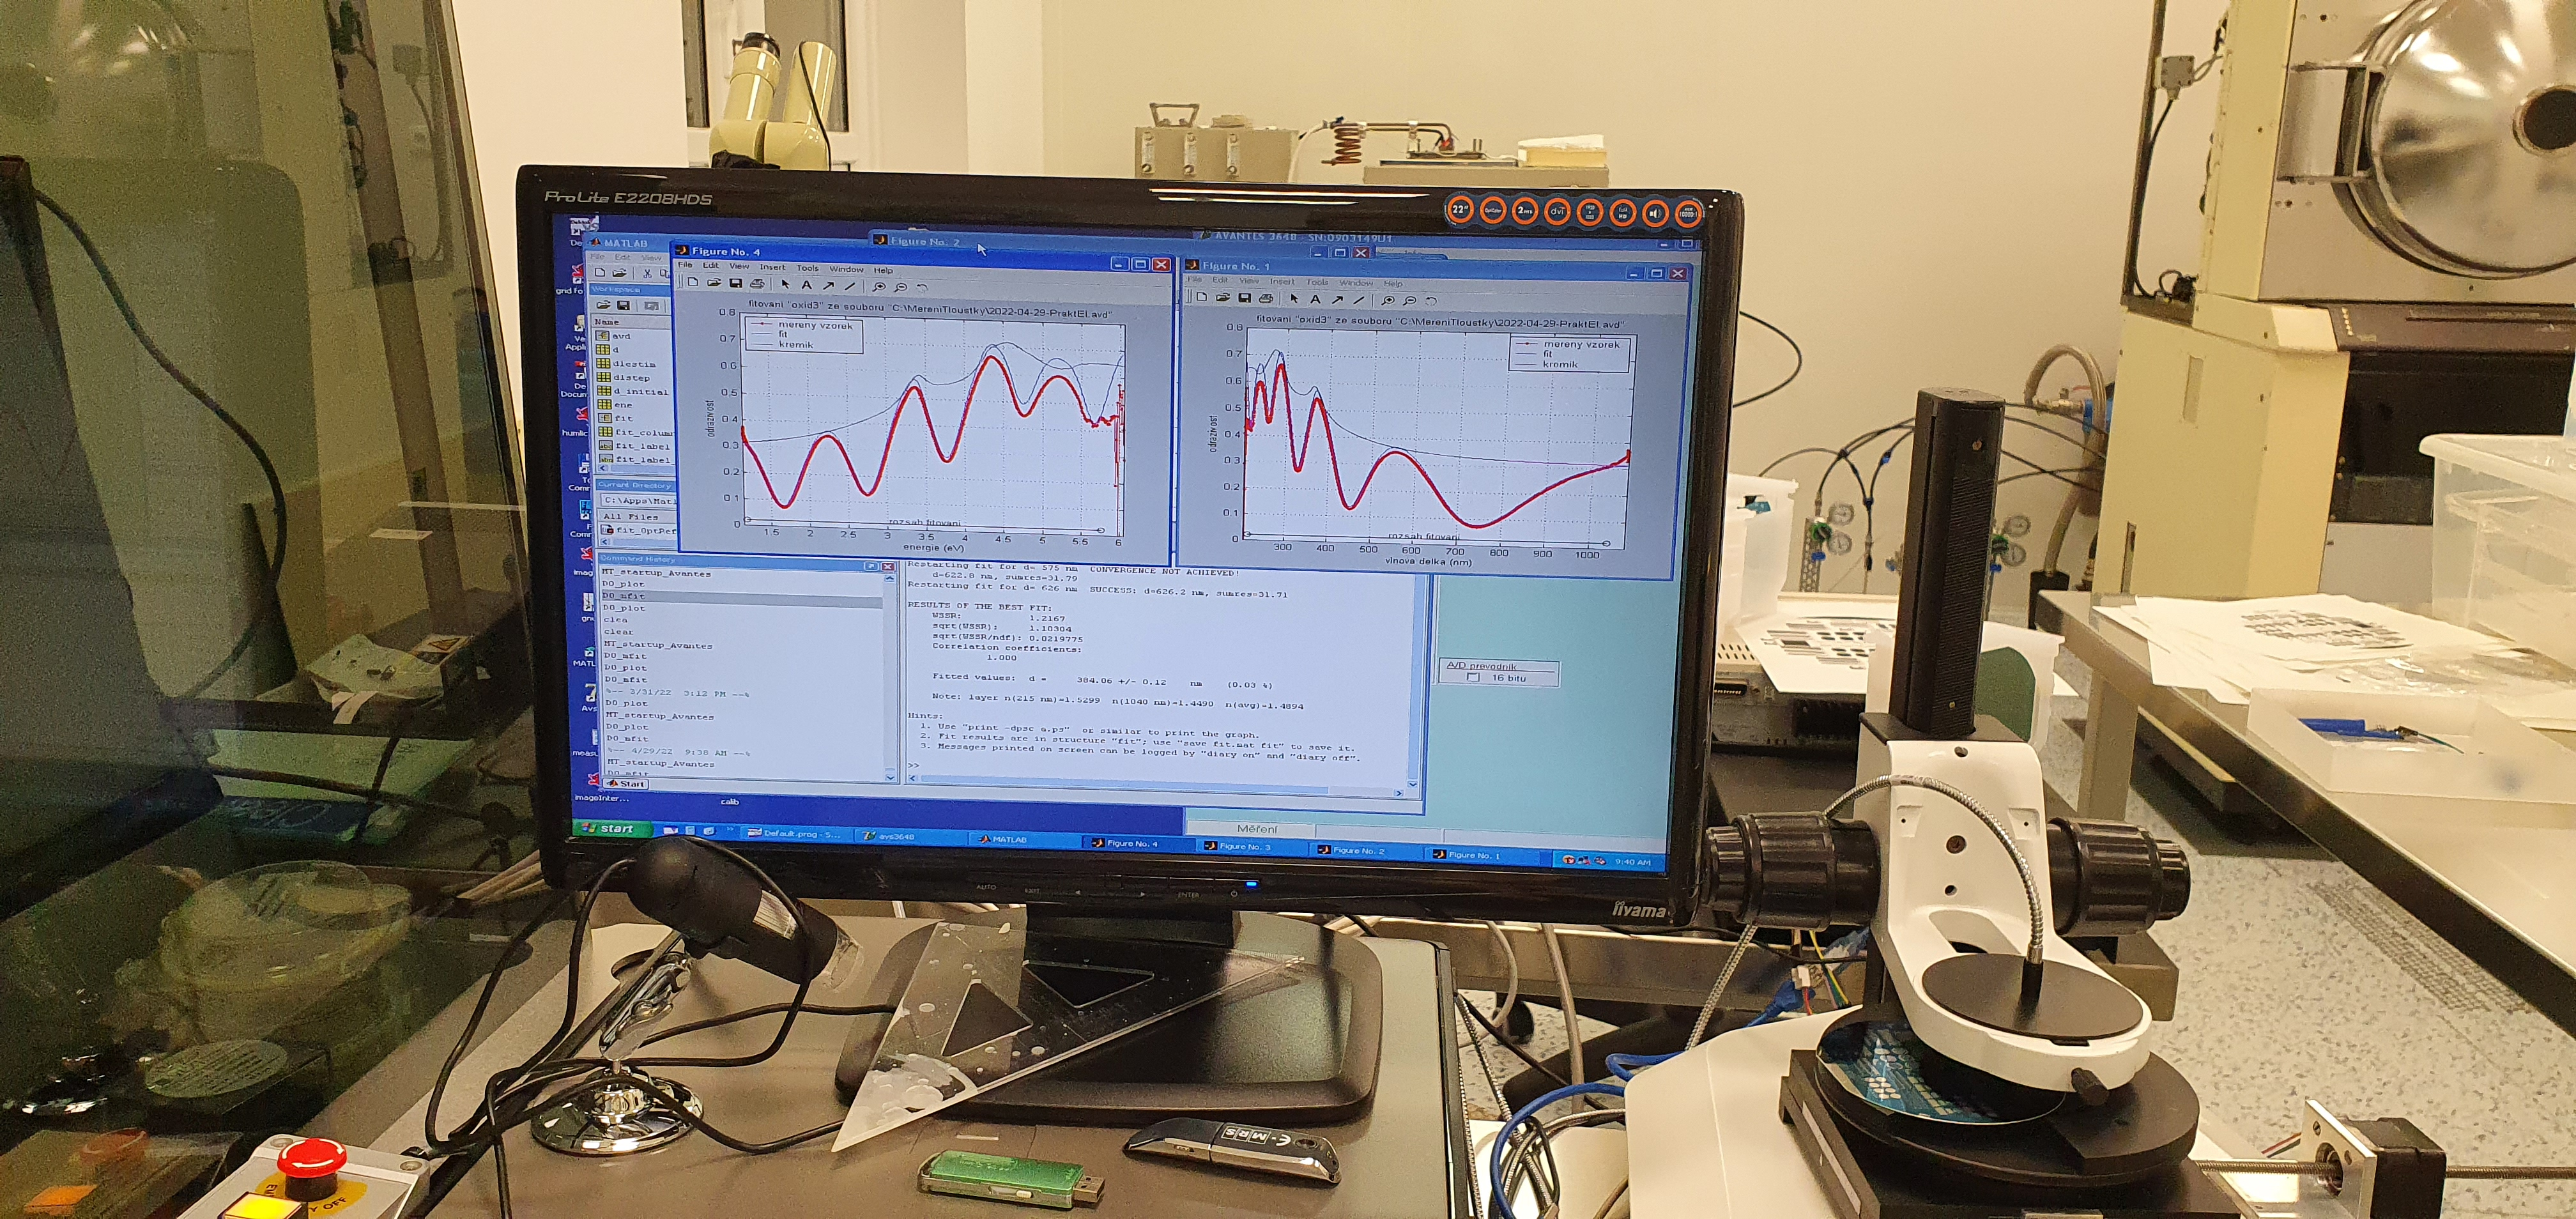
\includegraphics[width=130mm]{9interferometr.jpg}
	\caption{Měření interferometrem}
	\label{9interferometr}
\end{figure}

\begin{figure}[h!]
	\centering
	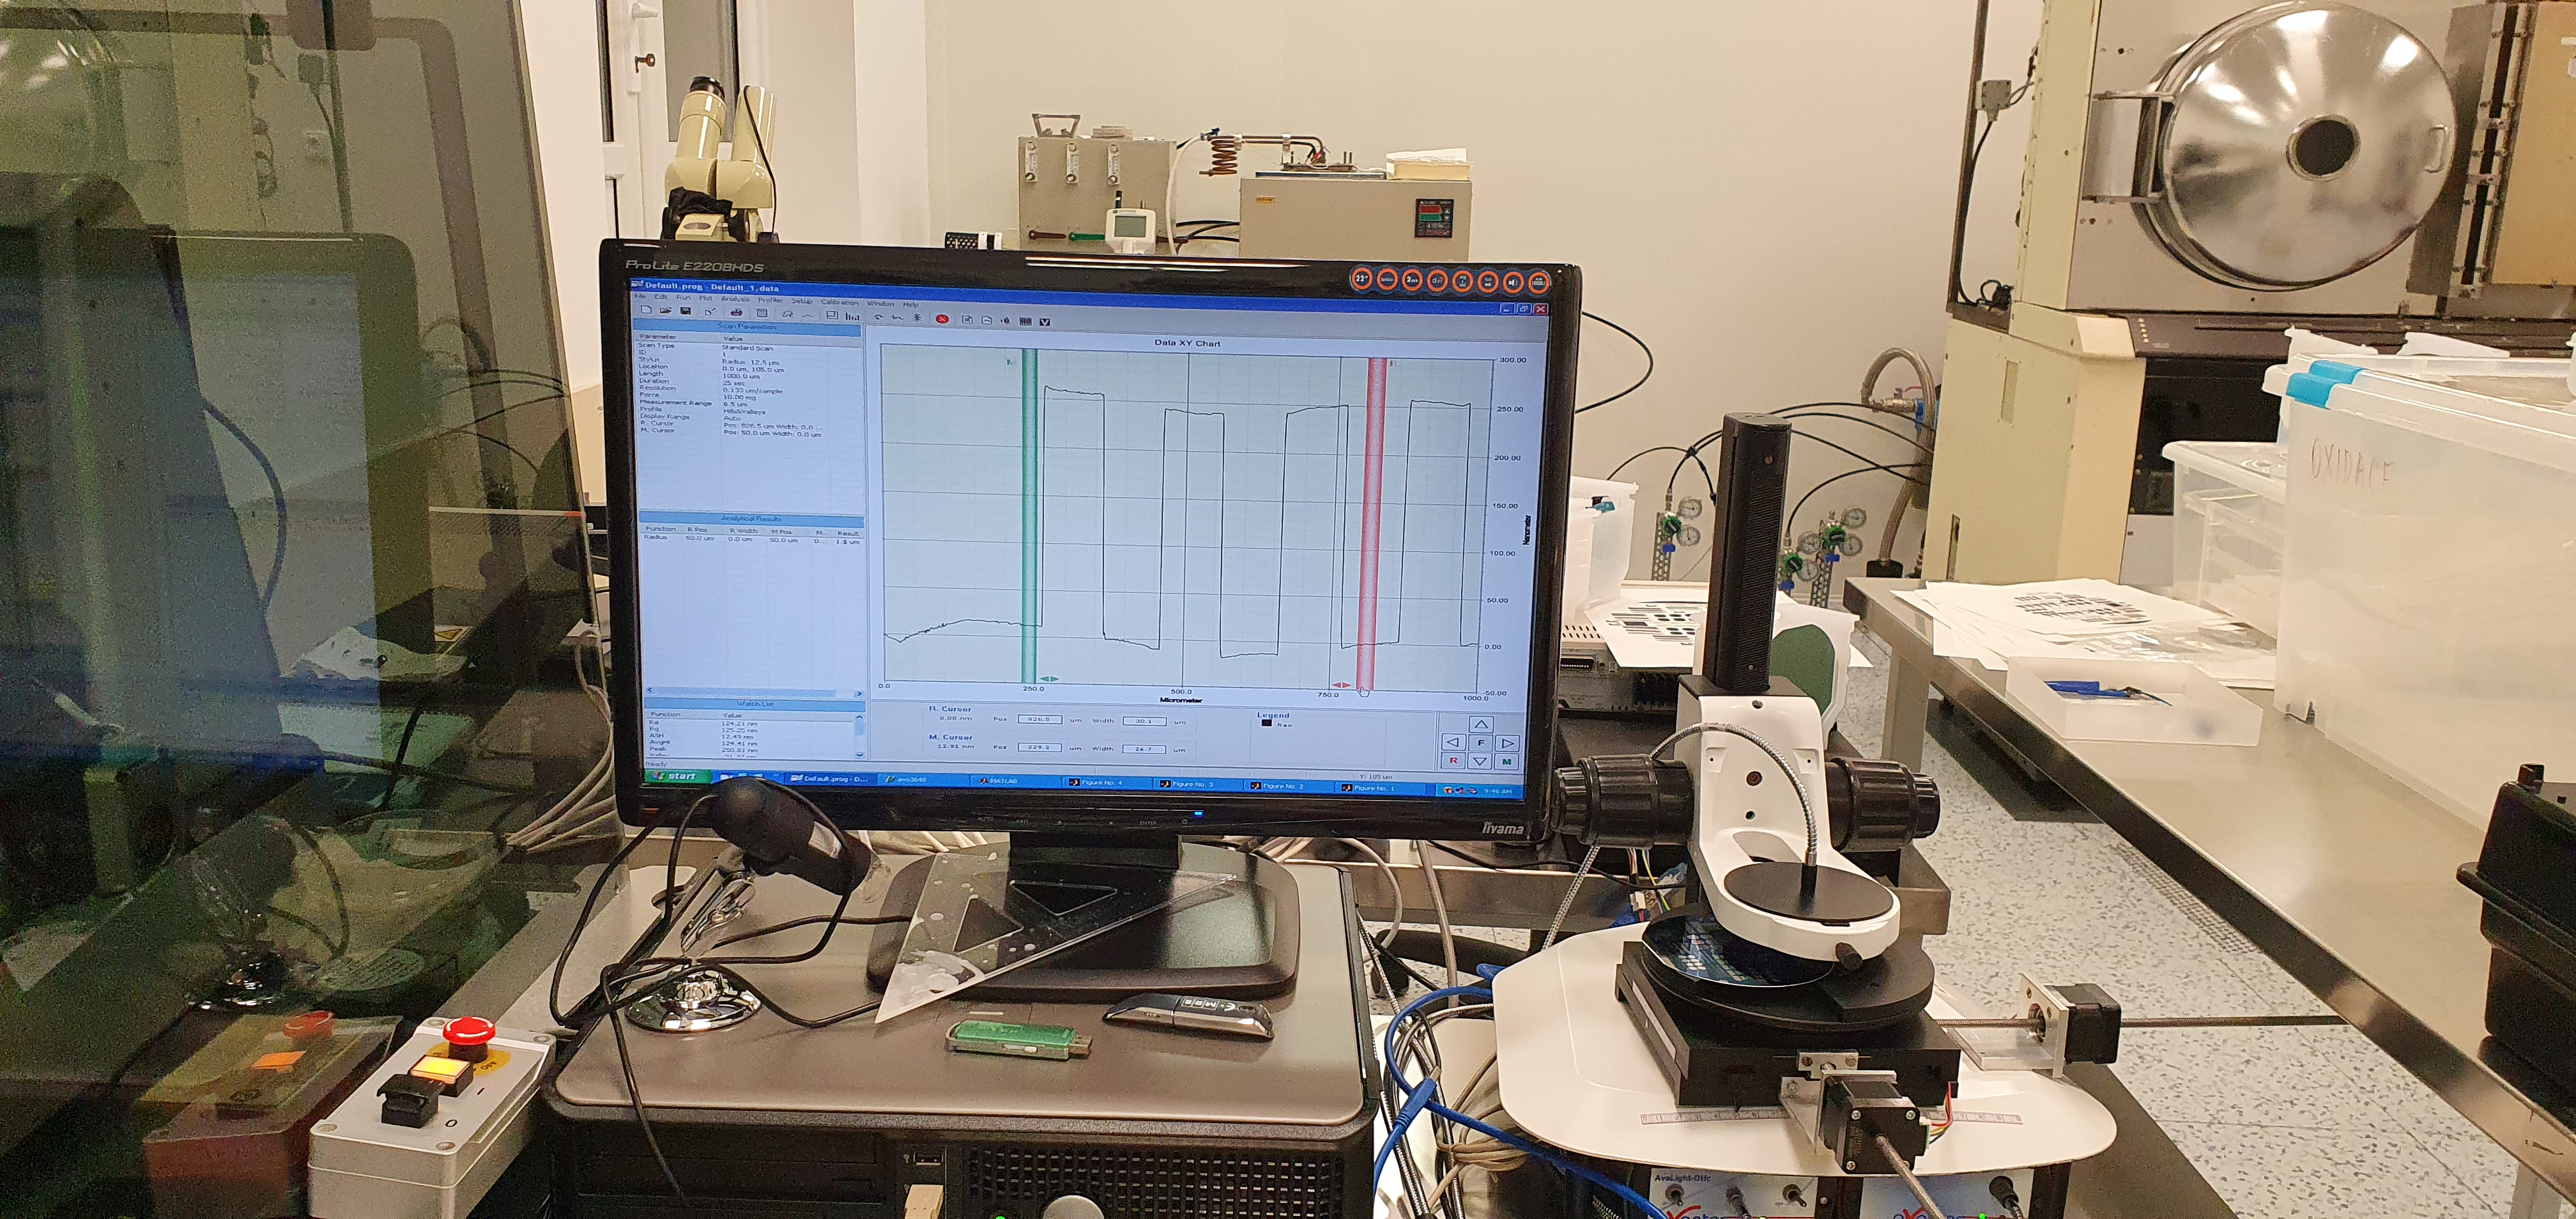
\includegraphics[width=130mm]{10profilometr.jpg}
	\caption{Měření profilometrem}
	\label{10profilometr}
\end{figure}

\section{Závěr}
V~rámci praktika v~čistých prostorách jsme se seznámili s~fotolitografickým 
procesem. Vyzkoušeli jsme si všechny jeho kroky a vyrobili křemíkovou desku
s~motivem obsahujícím rezistory a kondenzátory. Následně jsme u~některých z~nich 
naměřili odpory a kapacity. Tři rezistory měly odpor 382,6\,\si{\ohm}, 
450,6\,\si{\ohm} a 1,13\,\si{\kilo\ohm}. Dva kondenzátory měly kapacity 
380\,\si{\pico\farad} a 660\,\si{\pico\farad}. Nakonec jsme interferometrem 
provedli 
měření tloušťky SiO$_2$ vrstvy s~výslednou hodnotou 380\,\si{\nano\meter} a 
profilometrem jsme určili tloušťku hliníkové vrstvy  250\,\si{\nano\meter}.


\end{document}
